% !TEX TS-program = pdflatex
% !TEX encoding = UTF-8 Unicode
\documentclass[a4paper]{article}
\usepackage[swedish]{babel}
\usepackage[T1]{fontenc}
\usepackage[utf8]{inputenc}
\usepackage{mathtools}
\usepackage[pdftex]{graphicx}
\usepackage{float}
\usepackage{fancyhdr}
\usepackage{geometry}
\usepackage{booktabs} % for much better looking tables
\usepackage{array} % for better arrays (eg matrices) in maths
\usepackage{paralist} % very flexible & customisable lists (eg. enumerate/itemize, etc.)
\usepackage{verbatim} % adds environment for commenting out blocks of text & for better verbatim
\usepackage{subfig} % make it possible to include more than one captioned figure/table in a single float

%%% HEADERS & FOOTERS

\author{Jonathan Karlsson - jonka293 - 890201-1991 \and Niclas Olofsson - nicol271 - 900904-5338}
\pagestyle{fancy} % options: empty , plain , fancy
\renewcommand{\headrulewidth}{1pt} % customise the layout...
\fancyhead[LO,LE]{Laboration 3 - TDDC78}
\lfoot{}\cfoot{\thepage}\rfoot{}
\setlength{\parindent}{0pt}

%%%% SECTION TITLE APPEARANCE

%\usepackage{sectsty}
%\allsectionsfont{\sffamily\mdseries\upshape} % (See the fntguide.pdf for font help)
%% (This matches ConTeXt defaults)
%
%%%% ToC (table of contents) APPEARANCE
%\usepackage[nottoc,notlof,notlot]{tocbibind} % Put the bibliography in the ToC
%\usepackage[titles,subfigure]{tocloft} % Alter the style of the Table of Contents
%\renewcommand{\cftsecfont}{\rmfamily\mdseries\upshape}
%\renewcommand{\cftsecpagefont}{\rmfamily\mdseries\upshape} % No bold!

%%% END Article customizations

%%% The "real" document content comes below...

\title{Laboration 3 - TDDC78}

%\date{} % Activate to display a given date or no date (if empty),
% otherwise the current date is printed

\begin{document}

\maketitle

\section{Program description}
The program we got was using the Jacobi method to calculate temperatures on a quadratic plate. Basically what the method does is, for each point on the plate, calculate the temperature by adding the fore neighbors together.\\

Since fortran stores arrays column wise we want to iterate the plate column wise to save operation overhead. By identifying the dependencies in the program and saw that the last column can be written to at the same time as it is read by another node. We solved this by starting the parallel section, calculated  the interval each node should work on and with this we got what the first and last column was going to be.\\

Now we created a loop with \lq\lq{}maxiter\rq\rq{} iterations, in this loop we get the first and last column, make a barrier so each node has read the columns and now we create a new loop that iterates every column of the plate. Here openmp\rq{}s \lq\lq{}omp do\rq\rq{} is used to divide the columns into even work for each node. Inside this loop the regular Jacobi method is used with our previously read last column in the special case of then node being at the last iteration.\\

The reduction method is used to calculate the maximum error of each node, if this error is below our tolerance level then all nodes exit the loops and the program is done. The higher tolerance the better resolution but it will take significantly longer time.

\section{Execution times}
Below are figures showing the execution times. Figure \ref{fig:fig1} shows the execution times with two nodes, $maxiter = 1000$ and increasing $n = 100, 200, ..., 1600$. What we would like to see that if the problem size is doubled as well as the number of nodes we get a linear curve, this isn\rq{}t really achieved since we can\rq{}t simply double n and double the problem size since the plate have the dimensions $n * n$. But the figure shows that the result is somewhat linear so it tell us that the solution is probably correct.\\

Figure \ref{fig:fig2} shows the execution times with increasing number of nodes on the same problem size, $n = 1000$ and $maxiter = 1000$. This result is good with double amount of nodes gives half execution time, as expected.\\

 In figure \ref{fig:fig3} both the number of nodes and the problem size is increased. The point of this is to see a somewhat constant line, but again we have the problem with the problem size not really being doubled as with the number of nodes, but the result is still pretty close with the exception of $16$ and $32$ but that could be explained with bigger communication overhead over several processors.
 
\begin{figure}
  \centering
  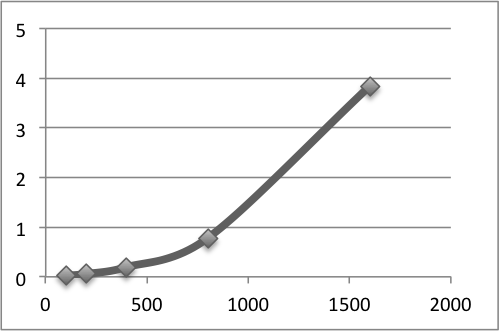
\includegraphics{samenodes.png}
  \caption{Execution times with two nodes, increasing problem size.}
  \label{fig:fig1}
\end{figure}

\begin{figure}
  \centering
  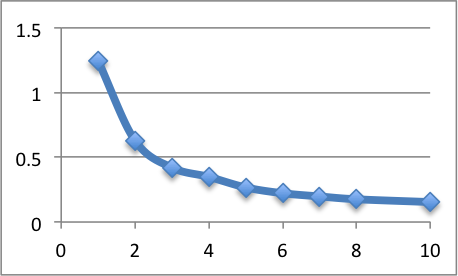
\includegraphics{lab3graph.png}
  \caption{Execution times on different number of nodes and same problem size.}
  \label{fig:fig2}
\end{figure}

\begin{figure}
  \centering
  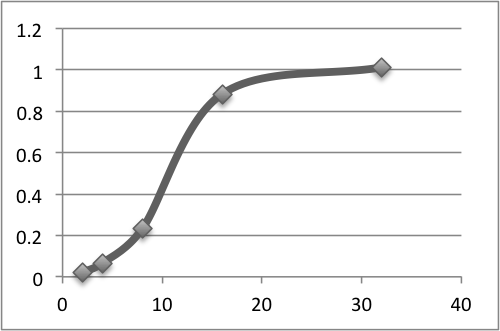
\includegraphics{samescale.png}
  \caption{Execution times with increasing number of nodes and an increasing problem size.}
  \label{fig:fig3}
\end{figure}
  

\end{document}
